\documentclass[twoside]{book}

% Packages required by doxygen
\usepackage{fixltx2e}
\usepackage{calc}
\usepackage{doxygen}
\usepackage[export]{adjustbox} % also loads graphicx
\usepackage{graphicx}
\usepackage[utf8]{inputenc}
\usepackage{makeidx}
\usepackage{multicol}
\usepackage{multirow}
\PassOptionsToPackage{warn}{textcomp}
\usepackage{textcomp}
\usepackage[nointegrals]{wasysym}
\usepackage[table]{xcolor}

% Font selection
\usepackage[T1]{fontenc}
\usepackage[scaled=.90]{helvet}
\usepackage{courier}
\usepackage{amssymb}
\usepackage{sectsty}
\renewcommand{\familydefault}{\sfdefault}
\allsectionsfont{%
  \fontseries{bc}\selectfont%
  \color{darkgray}%
}
\renewcommand{\DoxyLabelFont}{%
  \fontseries{bc}\selectfont%
  \color{darkgray}%
}
\newcommand{\+}{\discretionary{\mbox{\scriptsize$\hookleftarrow$}}{}{}}

% Page & text layout
\usepackage{geometry}
\geometry{%
  a4paper,%
  top=2.5cm,%
  bottom=2.5cm,%
  left=2.5cm,%
  right=2.5cm%
}
\tolerance=750
\hfuzz=15pt
\hbadness=750
\setlength{\emergencystretch}{15pt}
\setlength{\parindent}{0cm}
\setlength{\parskip}{3ex plus 2ex minus 2ex}
\makeatletter
\renewcommand{\paragraph}{%
  \@startsection{paragraph}{4}{0ex}{-1.0ex}{1.0ex}{%
    \normalfont\normalsize\bfseries\SS@parafont%
  }%
}
\renewcommand{\subparagraph}{%
  \@startsection{subparagraph}{5}{0ex}{-1.0ex}{1.0ex}{%
    \normalfont\normalsize\bfseries\SS@subparafont%
  }%
}
\makeatother

% Headers & footers
\usepackage{fancyhdr}
\pagestyle{fancyplain}
\fancyhead[LE]{\fancyplain{}{\bfseries\thepage}}
\fancyhead[CE]{\fancyplain{}{}}
\fancyhead[RE]{\fancyplain{}{\bfseries\leftmark}}
\fancyhead[LO]{\fancyplain{}{\bfseries\rightmark}}
\fancyhead[CO]{\fancyplain{}{}}
\fancyhead[RO]{\fancyplain{}{\bfseries\thepage}}
\fancyfoot[LE]{\fancyplain{}{}}
\fancyfoot[CE]{\fancyplain{}{}}
\fancyfoot[RE]{\fancyplain{}{\bfseries\scriptsize 產生者\+: Doxygen }}
\fancyfoot[LO]{\fancyplain{}{\bfseries\scriptsize 產生者\+: Doxygen }}
\fancyfoot[CO]{\fancyplain{}{}}
\fancyfoot[RO]{\fancyplain{}{}}
\renewcommand{\footrulewidth}{0.4pt}
\renewcommand{\chaptermark}[1]{%
  \markboth{#1}{}%
}
\renewcommand{\sectionmark}[1]{%
  \markright{\thesection\ #1}%
}

% Indices & bibliography
\usepackage{natbib}
\usepackage[titles]{tocloft}
\setcounter{tocdepth}{3}
\setcounter{secnumdepth}{5}
\makeindex

% Hyperlinks (required, but should be loaded last)
\usepackage{ifpdf}
\ifpdf
  \usepackage[pdftex,pagebackref=true]{hyperref}
\else
  \usepackage[ps2pdf,pagebackref=true]{hyperref}
\fi
\hypersetup{%
  colorlinks=true,%
  linkcolor=blue,%
  citecolor=blue,%
  unicode%
}

% Custom commands
\newcommand{\clearemptydoublepage}{%
  \newpage{\pagestyle{empty}\cleardoublepage}%
}

\usepackage{caption}
\captionsetup{labelsep=space,justification=centering,font={bf},singlelinecheck=off,skip=4pt,position=top}

%===== C O N T E N T S =====

\begin{document}

% Titlepage & ToC
\hypersetup{pageanchor=false,
             bookmarksnumbered=true,
             pdfencoding=unicode
            }
\pagenumbering{roman}
\begin{titlepage}
\vspace*{7cm}
\begin{center}%
{\Large Lexer }\\
\vspace*{1cm}
{\large 產生者\+: Doxygen 1.8.11}\\
\end{center}
\end{titlepage}
\clearemptydoublepage
\tableofcontents
\clearemptydoublepage
\pagenumbering{arabic}
\hypersetup{pageanchor=true}

%--- Begin generated contents ---
\chapter{命名空間(Namespace)索引}
\section{命名空間(name space)列表}
這是所有附帶簡略說明的命名空間(namespaces)\+:\begin{DoxyCompactList}
\item\contentsline{section}{\hyperlink{namespacelexer}{lexer} }{\pageref{namespacelexer}}{}
\end{DoxyCompactList}

\chapter{階層索引}
\section{類別階層}
這個繼承列表經過簡略的字母排序\+: \begin{DoxyCompactList}
\item \contentsline{section}{lexer.\+Lexer}{\pageref{classlexer_1_1_lexer}}{}
\item \contentsline{section}{lexer.\+Tag}{\pageref{classlexer_1_1_tag}}{}
\item \contentsline{section}{lexer.\+Token}{\pageref{classlexer_1_1_token}}{}
\begin{DoxyCompactList}
\item \contentsline{section}{lexer.\+Num}{\pageref{classlexer_1_1_num}}{}
\item \contentsline{section}{lexer.\+Word}{\pageref{classlexer_1_1_word}}{}
\end{DoxyCompactList}
\end{DoxyCompactList}

\chapter{複合索引}
\section{複合列表}
這是附帶簡略說明的類別,結構,聯合型態(unions)及介面(interfaces)\+:\begin{DoxyCompactList}
\item\contentsline{section}{\hyperlink{classlexer_1_1_lexer}{lexer.\+Lexer} }{\pageref{classlexer_1_1_lexer}}{}
\item\contentsline{section}{\hyperlink{classlexer_1_1_num}{lexer.\+Num} }{\pageref{classlexer_1_1_num}}{}
\item\contentsline{section}{\hyperlink{classlexer_1_1_tag}{lexer.\+Tag} }{\pageref{classlexer_1_1_tag}}{}
\item\contentsline{section}{\hyperlink{classlexer_1_1_token}{lexer.\+Token} }{\pageref{classlexer_1_1_token}}{}
\item\contentsline{section}{\hyperlink{classlexer_1_1_word}{lexer.\+Word} }{\pageref{classlexer_1_1_word}}{}
\end{DoxyCompactList}

\chapter{檔案索引}
\section{檔案列表}
這是附帶簡略說明的檔案列表\+:\begin{DoxyCompactList}
\item\contentsline{section}{\hyperlink{_lexer_8java}{Lexer.\+java} }{\pageref{_lexer_8java}}{}
\item\contentsline{section}{\hyperlink{_num_8java}{Num.\+java} }{\pageref{_num_8java}}{}
\item\contentsline{section}{\hyperlink{_tag_8java}{Tag.\+java} }{\pageref{_tag_8java}}{}
\item\contentsline{section}{\hyperlink{_token_8java}{Token.\+java} }{\pageref{_token_8java}}{}
\item\contentsline{section}{\hyperlink{_word_8java}{Word.\+java} }{\pageref{_word_8java}}{}
\end{DoxyCompactList}

\chapter{命名空間(Namespace)說明文件}
\hypertarget{namespacelexer}{}\section{Package lexer}
\label{namespacelexer}\index{lexer@{lexer}}
\subsection*{複合項目}
\begin{DoxyCompactItemize}
\item 
class \hyperlink{classlexer_1_1_lexer}{Lexer}
\item 
class \hyperlink{classlexer_1_1_num}{Num}
\item 
class \hyperlink{classlexer_1_1_tag}{Tag}
\item 
class \hyperlink{classlexer_1_1_token}{Token}
\item 
class \hyperlink{classlexer_1_1_word}{Word}
\end{DoxyCompactItemize}

\chapter{類別說明文件}
\hypertarget{classlexer_1_1_lexer}{}\section{lexer.\+Lexer 類別 參考文件}
\label{classlexer_1_1_lexer}\index{lexer.\+Lexer@{lexer.\+Lexer}}
\subsection*{公開方法(Public Methods)}
\begin{DoxyCompactItemize}
\item 
\hyperlink{classlexer_1_1_lexer_a74a5b43c328f1ed535ce18f4047e5eec}{Lexer} ()
\item 
\hyperlink{classlexer_1_1_token}{Token} \hyperlink{classlexer_1_1_lexer_a1f77e6a104c8d9f9c58aa303adfc9e9c}{scan} ()  throws I\+O\+Exception 
\end{DoxyCompactItemize}
\subsection*{公開屬性}
\begin{DoxyCompactItemize}
\item 
int \hyperlink{classlexer_1_1_lexer_aa3f0241bd211c220367e73def9003d94}{line} = 1
\end{DoxyCompactItemize}


\subsection{建構子與解構子說明文件}
\index{lexer\+::\+Lexer@{lexer\+::\+Lexer}!Lexer@{Lexer}}
\index{Lexer@{Lexer}!lexer\+::\+Lexer@{lexer\+::\+Lexer}}
\subsubsection[{\texorpdfstring{Lexer()}{Lexer()}}]{\setlength{\rightskip}{0pt plus 5cm}lexer.\+Lexer.\+Lexer (
\begin{DoxyParamCaption}
{}
\end{DoxyParamCaption}
)\hspace{0.3cm}{\ttfamily [inline]}}\hypertarget{classlexer_1_1_lexer_a74a5b43c328f1ed535ce18f4047e5eec}{}\label{classlexer_1_1_lexer_a74a5b43c328f1ed535ce18f4047e5eec}

\begin{DoxyCode}
15                    \{
16         reserve(\textcolor{keyword}{new} Word(Tag.TRUE, \textcolor{stringliteral}{"true"}));
17         reserve(\textcolor{keyword}{new} Word(Tag.FALSE, \textcolor{stringliteral}{"false"}));
18     \}
\end{DoxyCode}


\subsection{函式成員說明文件}
\index{lexer\+::\+Lexer@{lexer\+::\+Lexer}!scan@{scan}}
\index{scan@{scan}!lexer\+::\+Lexer@{lexer\+::\+Lexer}}
\subsubsection[{\texorpdfstring{scan()}{scan()}}]{\setlength{\rightskip}{0pt plus 5cm}{\bf Token} lexer.\+Lexer.\+scan (
\begin{DoxyParamCaption}
{}
\end{DoxyParamCaption}
) throws I\+O\+Exception\hspace{0.3cm}{\ttfamily [inline]}}\hypertarget{classlexer_1_1_lexer_a1f77e6a104c8d9f9c58aa303adfc9e9c}{}\label{classlexer_1_1_lexer_a1f77e6a104c8d9f9c58aa303adfc9e9c}

\begin{DoxyCode}
20                                            \{
21         \textcolor{keywordflow}{for} (; ; peek = (char) System.in.read()) \{
22             \textcolor{keywordflow}{if} (peek == \textcolor{charliteral}{' '} || peek == \textcolor{charliteral}{'\(\backslash\)t'}) \textcolor{keywordflow}{continue};
23             \textcolor{keywordflow}{else} \textcolor{keywordflow}{if} (peek == \textcolor{charliteral}{'\(\backslash\)n'}) \hyperlink{classlexer_1_1_lexer_aa3f0241bd211c220367e73def9003d94}{line}++;
24             \textcolor{keywordflow}{else} \textcolor{keywordflow}{break};
25         \}
26 
27         \textcolor{keywordflow}{if} (Character.isDigit(peek)) \{
28             \textcolor{keywordtype}{int} v = 0;
29             \textcolor{keywordflow}{do} \{
30                 v = 10 * v + Character.digit(peek, 10);
31                 peek = (char) System.in.read();
32             \} \textcolor{keywordflow}{while} (Character.isDigit(peek));
33 
34             \textcolor{keywordflow}{return} \textcolor{keyword}{new} Num(v);
35         \}
36 
37         \textcolor{keywordflow}{if} (Character.isLetter(peek)) \{
38             StringBuffer b = \textcolor{keyword}{new} StringBuffer();
39             \textcolor{keywordflow}{do} \{
40                 b.append(peek);
41                 peek = (char) System.in.read();
42             \} \textcolor{keywordflow}{while} (Character.isLetterOrDigit(peek));
43 
44             String s = b.toString();
45             Word w = (Word) words.get(s);
46             \textcolor{keywordflow}{if} (w != null) \textcolor{keywordflow}{return} w;
47             w = \textcolor{keyword}{new} Word(Tag.ID, s);
48             words.put(s, w);
49             \textcolor{keywordflow}{return} w;
50         \}
51 
52         Token t = \textcolor{keyword}{new} Token(peek);
53         peek = \textcolor{charliteral}{' '};
54         \textcolor{keywordflow}{return} t;
55     \}
\end{DoxyCode}


\subsection{資料成員說明文件}
\index{lexer\+::\+Lexer@{lexer\+::\+Lexer}!line@{line}}
\index{line@{line}!lexer\+::\+Lexer@{lexer\+::\+Lexer}}
\subsubsection[{\texorpdfstring{line}{line}}]{\setlength{\rightskip}{0pt plus 5cm}int lexer.\+Lexer.\+line = 1}\hypertarget{classlexer_1_1_lexer_aa3f0241bd211c220367e73def9003d94}{}\label{classlexer_1_1_lexer_aa3f0241bd211c220367e73def9003d94}


此類別(class) 文件是由下列檔案中產生\+:\begin{DoxyCompactItemize}
\item 
\hyperlink{_lexer_8java}{Lexer.\+java}\end{DoxyCompactItemize}

\hypertarget{classlexer_1_1_num}{}\section{lexer.\+Num 類別 參考文件}
\label{classlexer_1_1_num}\index{lexer.\+Num@{lexer.\+Num}}
類別lexer.\+Num的繼承圖\+:\begin{figure}[H]
\begin{center}
\leavevmode
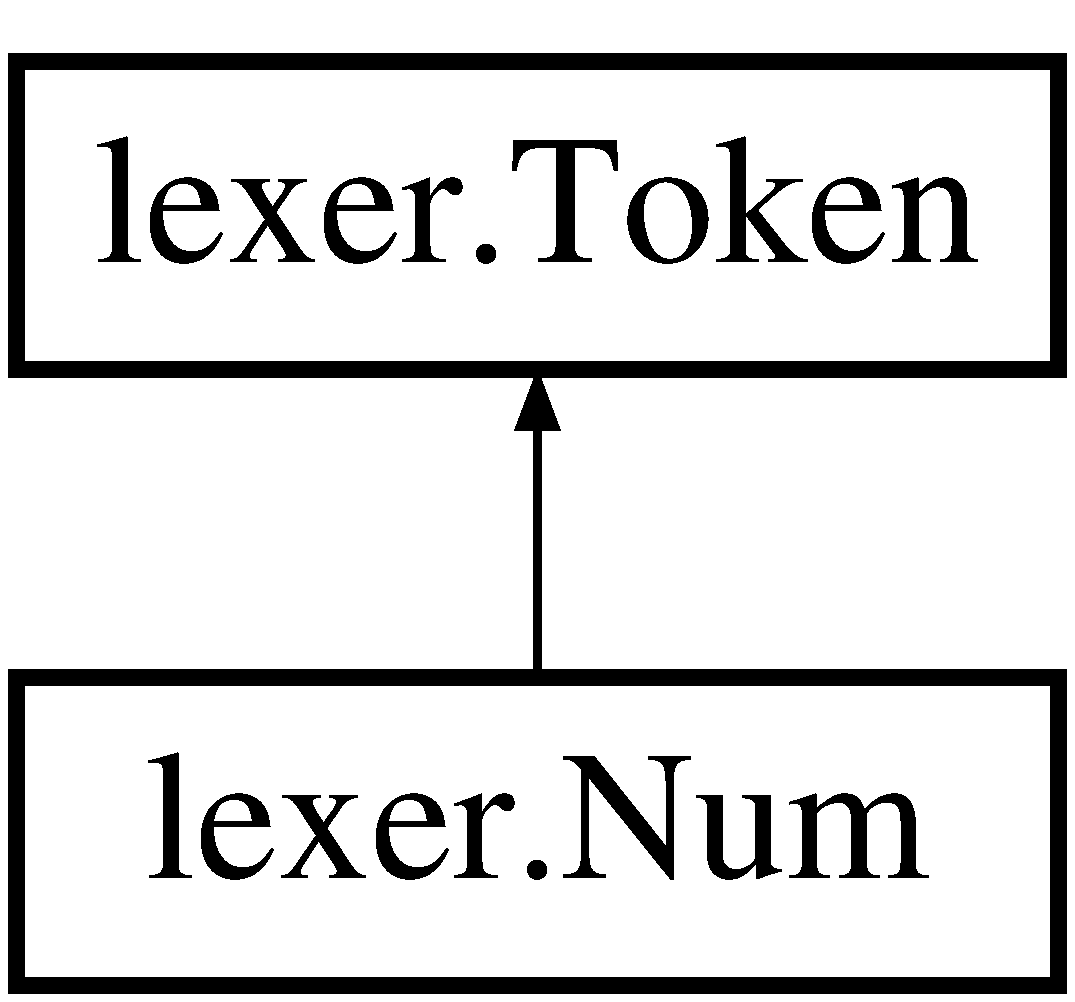
\includegraphics[height=2.000000cm]{classlexer_1_1_num}
\end{center}
\end{figure}
\subsection*{公開方法(Public Methods)}
\begin{DoxyCompactItemize}
\item 
\hyperlink{classlexer_1_1_num_a6b042277c09487a070b5305857827ef0}{Num} (int v)
\end{DoxyCompactItemize}
\subsection*{公開屬性}
\begin{DoxyCompactItemize}
\item 
final int \hyperlink{classlexer_1_1_num_a38cc342dd32da91084432bb0c338b8b0}{value}
\end{DoxyCompactItemize}


\subsection{建構子與解構子說明文件}
\index{lexer\+::\+Num@{lexer\+::\+Num}!Num@{Num}}
\index{Num@{Num}!lexer\+::\+Num@{lexer\+::\+Num}}
\subsubsection[{\texorpdfstring{Num(int v)}{Num(int v)}}]{\setlength{\rightskip}{0pt plus 5cm}lexer.\+Num.\+Num (
\begin{DoxyParamCaption}
\item[{int}]{v}
\end{DoxyParamCaption}
)\hspace{0.3cm}{\ttfamily [inline]}}\hypertarget{classlexer_1_1_num_a6b042277c09487a070b5305857827ef0}{}\label{classlexer_1_1_num_a6b042277c09487a070b5305857827ef0}

\begin{DoxyCode}
5                       \{
6         super(Tag.NUM);
7         \hyperlink{classlexer_1_1_num_a38cc342dd32da91084432bb0c338b8b0}{value}=v;
8     \}
\end{DoxyCode}


\subsection{資料成員說明文件}
\index{lexer\+::\+Num@{lexer\+::\+Num}!value@{value}}
\index{value@{value}!lexer\+::\+Num@{lexer\+::\+Num}}
\subsubsection[{\texorpdfstring{value}{value}}]{\setlength{\rightskip}{0pt plus 5cm}final int lexer.\+Num.\+value}\hypertarget{classlexer_1_1_num_a38cc342dd32da91084432bb0c338b8b0}{}\label{classlexer_1_1_num_a38cc342dd32da91084432bb0c338b8b0}


此類別(class) 文件是由下列檔案中產生\+:\begin{DoxyCompactItemize}
\item 
\hyperlink{_num_8java}{Num.\+java}\end{DoxyCompactItemize}

\hypertarget{classlexer_1_1_tag}{}\section{lexer.\+Tag 類別 參考文件}
\label{classlexer_1_1_tag}\index{lexer.\+Tag@{lexer.\+Tag}}
\subsection*{靜態公開屬性}
\begin{DoxyCompactItemize}
\item 
static final int \hyperlink{classlexer_1_1_tag_aafbd77c472e395e2fd5cce9f772bca75}{N\+UM} =256
\end{DoxyCompactItemize}


\subsection{詳細描述}
Created by U\+S\+ER on 2016/8/27. 

\subsection{資料成員說明文件}
\index{lexer\+::\+Tag@{lexer\+::\+Tag}!N\+UM@{N\+UM}}
\index{N\+UM@{N\+UM}!lexer\+::\+Tag@{lexer\+::\+Tag}}
\subsubsection[{\texorpdfstring{N\+UM}{NUM}}]{\setlength{\rightskip}{0pt plus 5cm}final int lexer.\+Tag.\+N\+UM =256\hspace{0.3cm}{\ttfamily [static]}}\hypertarget{classlexer_1_1_tag_aafbd77c472e395e2fd5cce9f772bca75}{}\label{classlexer_1_1_tag_aafbd77c472e395e2fd5cce9f772bca75}


此類別(class) 文件是由下列檔案中產生\+:\begin{DoxyCompactItemize}
\item 
\hyperlink{_tag_8java}{Tag.\+java}\end{DoxyCompactItemize}

\hypertarget{classlexer_1_1_token}{}\section{lexer.\+Token 類別 參考文件}
\label{classlexer_1_1_token}\index{lexer.\+Token@{lexer.\+Token}}
類別lexer.\+Token的繼承圖\+:\begin{figure}[H]
\begin{center}
\leavevmode
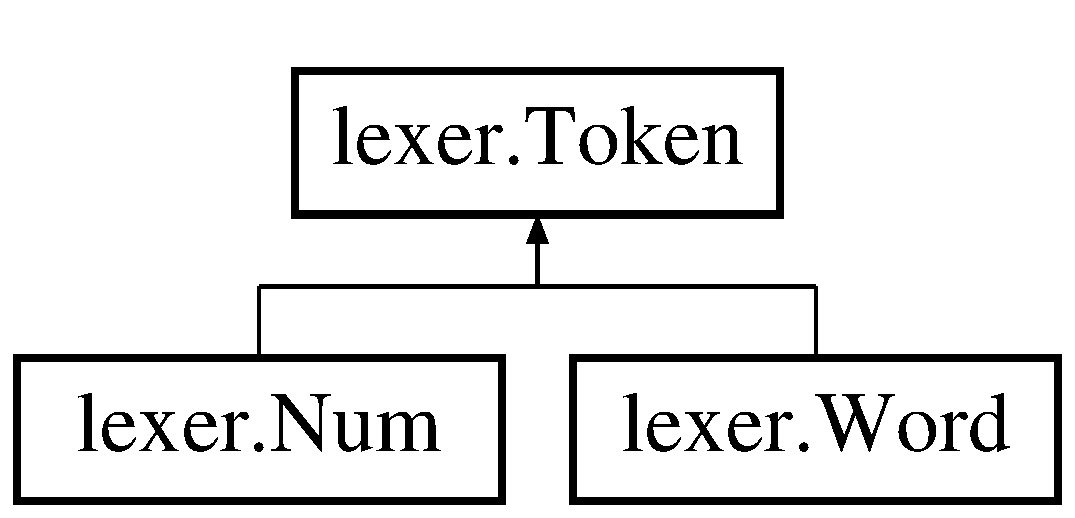
\includegraphics[height=2.000000cm]{classlexer_1_1_token}
\end{center}
\end{figure}
\subsection*{公開方法(Public Methods)}
\begin{DoxyCompactItemize}
\item 
\hyperlink{classlexer_1_1_token_afa1b0abde90efa5c33a97eea37c9bef4}{Token} (int t)
\end{DoxyCompactItemize}
\subsection*{公開屬性}
\begin{DoxyCompactItemize}
\item 
final int \hyperlink{classlexer_1_1_token_a53e09da48c3c975277779c52b3597606}{tag}
\end{DoxyCompactItemize}


\subsection{建構子與解構子說明文件}
\index{lexer\+::\+Token@{lexer\+::\+Token}!Token@{Token}}
\index{Token@{Token}!lexer\+::\+Token@{lexer\+::\+Token}}
\subsubsection[{\texorpdfstring{Token(int t)}{Token(int t)}}]{\setlength{\rightskip}{0pt plus 5cm}lexer.\+Token.\+Token (
\begin{DoxyParamCaption}
\item[{int}]{t}
\end{DoxyParamCaption}
)\hspace{0.3cm}{\ttfamily [inline]}}\hypertarget{classlexer_1_1_token_afa1b0abde90efa5c33a97eea37c9bef4}{}\label{classlexer_1_1_token_afa1b0abde90efa5c33a97eea37c9bef4}

\begin{DoxyCode}
4                         \{
5         \hyperlink{classlexer_1_1_token_a53e09da48c3c975277779c52b3597606}{tag}=t;
6     \}
\end{DoxyCode}


\subsection{資料成員說明文件}
\index{lexer\+::\+Token@{lexer\+::\+Token}!tag@{tag}}
\index{tag@{tag}!lexer\+::\+Token@{lexer\+::\+Token}}
\subsubsection[{\texorpdfstring{tag}{tag}}]{\setlength{\rightskip}{0pt plus 5cm}final int lexer.\+Token.\+tag}\hypertarget{classlexer_1_1_token_a53e09da48c3c975277779c52b3597606}{}\label{classlexer_1_1_token_a53e09da48c3c975277779c52b3597606}


此類別(class) 文件是由下列檔案中產生\+:\begin{DoxyCompactItemize}
\item 
\hyperlink{_token_8java}{Token.\+java}\end{DoxyCompactItemize}

\hypertarget{classlexer_1_1_word}{}\section{lexer.\+Word 類別 參考文件}
\label{classlexer_1_1_word}\index{lexer.\+Word@{lexer.\+Word}}
類別lexer.\+Word的繼承圖\+:\begin{figure}[H]
\begin{center}
\leavevmode
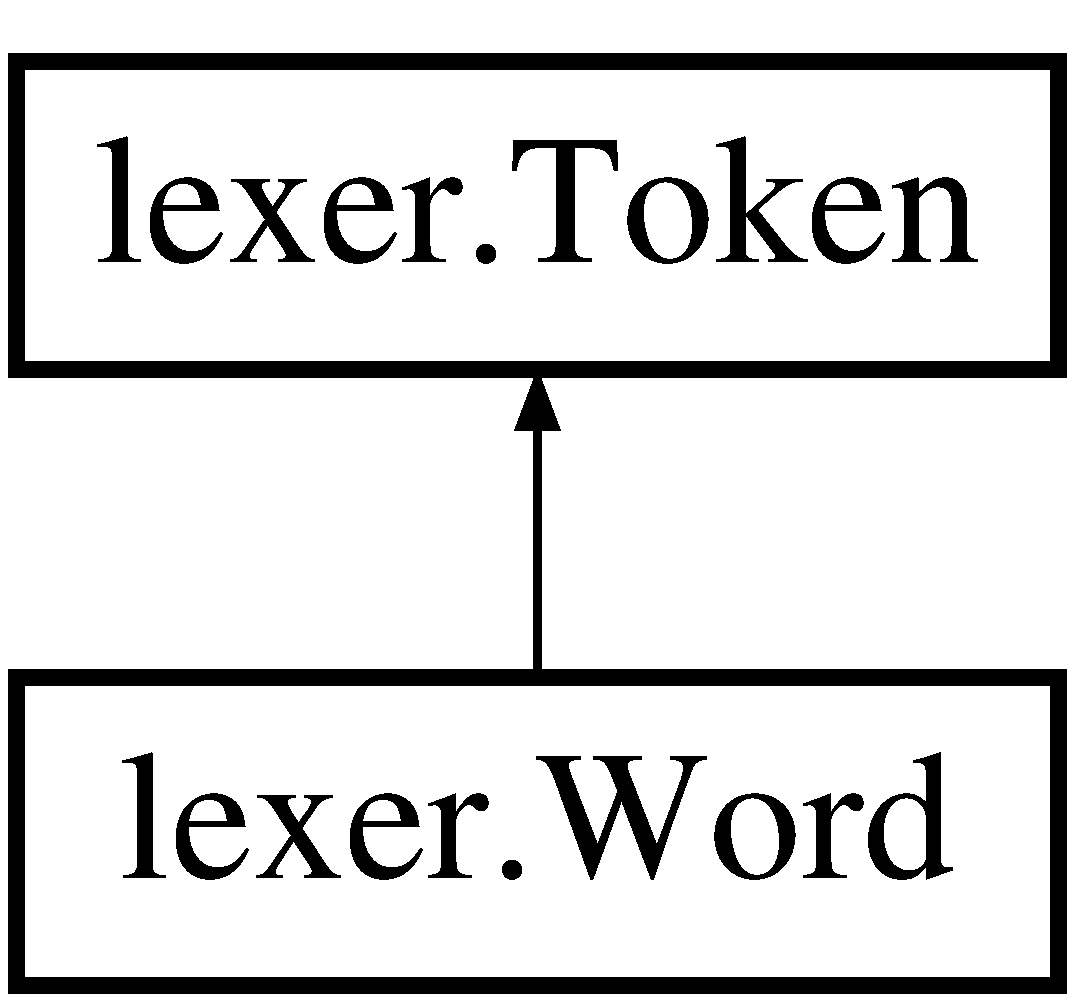
\includegraphics[height=2.000000cm]{classlexer_1_1_word}
\end{center}
\end{figure}
\subsection*{公開方法(Public Methods)}
\begin{DoxyCompactItemize}
\item 
\hyperlink{classlexer_1_1_word_af226bc11561fc611692f41355e2a2e92}{Word} (int t, String s)
\end{DoxyCompactItemize}
\subsection*{公開屬性}
\begin{DoxyCompactItemize}
\item 
final String \hyperlink{classlexer_1_1_word_a9e398a2a4009ed6a16bdee2d90a34dcf}{lexeme}
\end{DoxyCompactItemize}


\subsection{建構子與解構子說明文件}
\index{lexer\+::\+Word@{lexer\+::\+Word}!Word@{Word}}
\index{Word@{Word}!lexer\+::\+Word@{lexer\+::\+Word}}
\subsubsection[{\texorpdfstring{Word(int t, String s)}{Word(int t, String s)}}]{\setlength{\rightskip}{0pt plus 5cm}lexer.\+Word.\+Word (
\begin{DoxyParamCaption}
\item[{int}]{t, }
\item[{String}]{s}
\end{DoxyParamCaption}
)\hspace{0.3cm}{\ttfamily [inline]}}\hypertarget{classlexer_1_1_word_af226bc11561fc611692f41355e2a2e92}{}\label{classlexer_1_1_word_af226bc11561fc611692f41355e2a2e92}

\begin{DoxyCode}
6                                  \{
7         super(t);
8         \hyperlink{classlexer_1_1_word_a9e398a2a4009ed6a16bdee2d90a34dcf}{lexeme} = \textcolor{keyword}{new} String(s);
9     \}
\end{DoxyCode}


\subsection{資料成員說明文件}
\index{lexer\+::\+Word@{lexer\+::\+Word}!lexeme@{lexeme}}
\index{lexeme@{lexeme}!lexer\+::\+Word@{lexer\+::\+Word}}
\subsubsection[{\texorpdfstring{lexeme}{lexeme}}]{\setlength{\rightskip}{0pt plus 5cm}final String lexer.\+Word.\+lexeme}\hypertarget{classlexer_1_1_word_a9e398a2a4009ed6a16bdee2d90a34dcf}{}\label{classlexer_1_1_word_a9e398a2a4009ed6a16bdee2d90a34dcf}


此類別(class) 文件是由下列檔案中產生\+:\begin{DoxyCompactItemize}
\item 
\hyperlink{_word_8java}{Word.\+java}\end{DoxyCompactItemize}

\chapter{檔案說明文件}
\hypertarget{_lexer_8java}{}\section{Lexer.\+java 檔案參考文件}
\label{_lexer_8java}\index{Lexer.\+java@{Lexer.\+java}}
\subsection*{複合項目}
\begin{DoxyCompactItemize}
\item 
class \hyperlink{classlexer_1_1_lexer}{lexer.\+Lexer}
\end{DoxyCompactItemize}
\subsection*{Packages}
\begin{DoxyCompactItemize}
\item 
package \hyperlink{namespacelexer}{lexer}
\end{DoxyCompactItemize}

\hypertarget{_num_8java}{}\section{Num.\+java 檔案參考文件}
\label{_num_8java}\index{Num.\+java@{Num.\+java}}
\subsection*{複合項目}
\begin{DoxyCompactItemize}
\item 
class \hyperlink{classlexer_1_1_num}{lexer.\+Num}
\end{DoxyCompactItemize}
\subsection*{Packages}
\begin{DoxyCompactItemize}
\item 
package \hyperlink{namespacelexer}{lexer}
\end{DoxyCompactItemize}

\hypertarget{_tag_8java}{}\section{Tag.\+java 檔案參考文件}
\label{_tag_8java}\index{Tag.\+java@{Tag.\+java}}
\subsection*{複合項目}
\begin{DoxyCompactItemize}
\item 
class \hyperlink{classlexer_1_1_tag}{lexer.\+Tag}
\end{DoxyCompactItemize}
\subsection*{Packages}
\begin{DoxyCompactItemize}
\item 
package \hyperlink{namespacelexer}{lexer}
\end{DoxyCompactItemize}

\hypertarget{_token_8java}{}\section{Token.\+java 檔案參考文件}
\label{_token_8java}\index{Token.\+java@{Token.\+java}}
\subsection*{複合項目}
\begin{DoxyCompactItemize}
\item 
class \hyperlink{classlexer_1_1_token}{lexer.\+Token}
\end{DoxyCompactItemize}
\subsection*{Packages}
\begin{DoxyCompactItemize}
\item 
package \hyperlink{namespacelexer}{lexer}
\end{DoxyCompactItemize}

\hypertarget{_word_8java}{}\section{Word.\+java 檔案參考文件}
\label{_word_8java}\index{Word.\+java@{Word.\+java}}
\subsection*{複合項目}
\begin{DoxyCompactItemize}
\item 
class \hyperlink{classlexer_1_1_word}{lexer.\+Word}
\end{DoxyCompactItemize}
\subsection*{Packages}
\begin{DoxyCompactItemize}
\item 
package \hyperlink{namespacelexer}{lexer}
\end{DoxyCompactItemize}

%--- End generated contents ---

% Index
\backmatter
\newpage
\phantomsection
\clearemptydoublepage
\addcontentsline{toc}{chapter}{索引}
\printindex

\end{document}
